\documentclass[sectionformat = exercise]{gadsescript}
\settitle{Exercise Sheet 3}
\setsubtitle{Elias Gestrich}

\begin{document}
\maketitle
\section{Lists and Arrays}
\begin{enumerate}[label=\alph*)]
	\item iii)
	\item ii)
\end{enumerate}

\section{Stacks}
\begin{enumerate}[label=\alph*)]
	\item The array $[(]$ and the array $[(, (, )]$ result in a return of $true$, but they are no correct sequences of parantheses.
	\item One can insert
		\begin{algorithm*}
			\textbf{if not} \textit{S.isEmpty()} \textbf{then}\\
			\quad \textbf{return} \textit{false}
		\end{algorithm*}
		between line 8 and 9
\end{enumerate}

\section{Graphs}
\begin{enumerate}[label=\alph*)]
	\item ~\\
		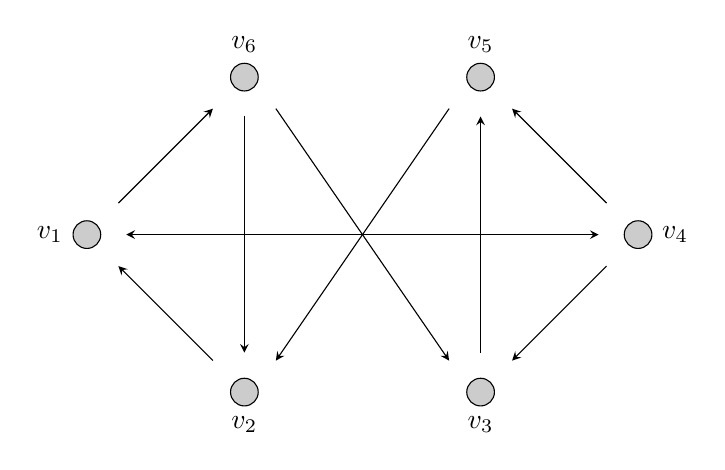
\begin{tikzpicture}
			\node[fill, fill opacity = 0.2, draw, circle, label=left: $v_1$, inner sep = 0, minimum size = 10] at (0,0) {};
			\node[fill, fill opacity = 0.2, draw, circle, label=above: $v_6$, inner sep = 0, minimum size = 10] at (2,2) {};
			\node[fill, fill opacity = 0.2, draw, circle, label=below: $v_2$, inner sep = 0, minimum size = 10] at (2,-2) {};
			\node[fill, fill opacity = 0.2, draw, circle, label=above: $v_5$, inner sep = 0, minimum size = 10] at (5,2) {};
			\node[fill, fill opacity = 0.2, draw, circle, label=below: $v_3$, inner sep = 0, minimum size = 10] at (5,-2) {};
			\node[fill, fill opacity = 0.2, draw, circle, label=right: $v_4$, inner sep = 0, minimum size = 10] at (7,0) {};
			\draw[stealth-stealth] (0.5, 0) -- (6.5,0);
			\draw[-stealth] (0.4, 0.4) -- (1.6,1.6);
			\draw[-stealth] (1.6, -1.6) -- (0.4,-0.4);
			\draw[-stealth] (5, -1.5) -- (5, 1.5);
			\draw[-stealth] (6.6, -0.4) -- (5.4, -1.6);
			\draw[-stealth] (6.6, 0.4) -- (5.4, 1.6);
			\draw[-stealth] (4.6, 1.6) -- (2.4, -1.6);
			\draw[-stealth] (2, 1.5) -- (2, -1.5);
			\draw[-stealth] (2.4, 1.6) -- (4.6, -1.6);
		\end{tikzpicture}
	\item ~\\
		\begin{tabular}{c||c|c|c}
			$v_1$ & $v_4$ & $ v_6 $ &~\\\hline
			$v_2$ & $v_1$ & ~ &~\\\hline
			$v_3$ & $v_5$ & ~ &~\\\hline
			$v_4$ & $v_1$ & $ v_3 $ & $ v_5$\\\hline
			$v_5$ & $v_2$ & ~ &~\\\hline
			$v_6$ & $v_2$ & $ v_3 $ &~\\
		\end{tabular}
\end{enumerate}

\end{document}
